\subsection{What is an address?}
\label{subsect:def_adresses}

An address is primarily an indirect spatial reference, a structured statement that designates a location unambiguously~\cite{coetzee_towards_2011}.
Although the form and nature of what it designates vary depending on periods and locations,~\cite{morita_cheminement_1980} identifies two categories.
The administrative address, which only defines the position of a place, differs from the itinerary address, which describes a path through space.
"\textit{59 rue de Rivoli, 75001 Paris}" and "\textit{maison de la Belle-Jardinière, quai aux Fleurs, coin de la rue de la Cité}" are respectively examples of these two address categories.
An address is therefore a composite entity, made of spatial references organized into hierarchies and whose spatial relationships may be explicitly described~\cite{coetzee_towards_2011}.
These components are spatial landmarks, possibly informal, known and shared by the people using the address~\cite{dumedah_address_2021}.
In this article, an address is therefore defined as a structured statement describing a path within a spatial hierarchy, unambiguous within this hierarchy, composed of an ordered sequence of spatial landmarks whose conceptualization and designation are known and shared.

\subsection{Addressing systems in Paris since the 18\textsuperscript{th} century}
\label{subsect:histoire_adresses_paris}

\begin{figure}[ht]
     \centering
     \begin{subfigure}[b]{0.32\textwidth}
         \centering
         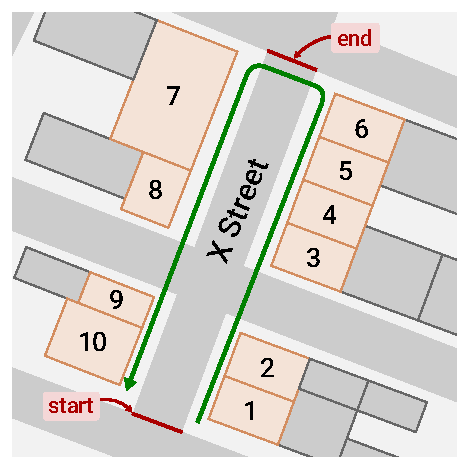
\includegraphics[width=\textwidth]{images/systemes_numerotation_paris_royal.pdf}
         \caption{Kreenfelt system}
         \label{fig:systemes_numerotation_paris_royal}
     \end{subfigure}
     \hfill
     \begin{subfigure}[b]{0.32\textwidth}
         \centering
         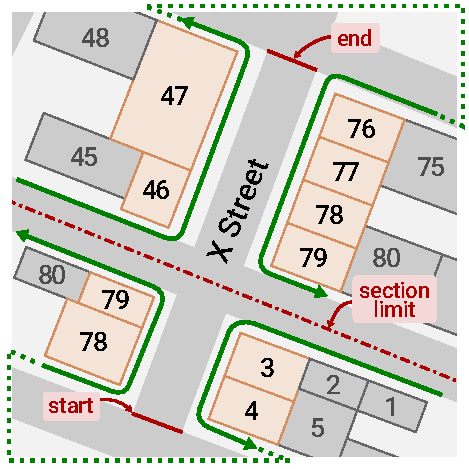
\includegraphics[width=\textwidth]{images/systemes_numerotation_paris_revolutionnaire.pdf}
         \caption{Revolutionary system}
         \label{fig:systemes_numerotation_paris_revolutionnaire}
     \end{subfigure}
     \hfill
     \begin{subfigure}[b]{0.32\textwidth}
         \centering
         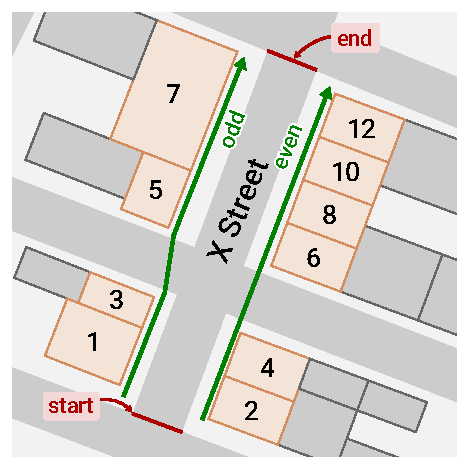
\includegraphics[width=\textwidth]{images/systemes_numerotation_paris_imperial.pdf}
         \caption{Imperial system}
         \label{fig:systemes_numerotation_paris_imperial}
     \end{subfigure}
     \caption{The three house numbering systems used in Paris. Green arrows indicate the numbering direction.}
     \label{fig:systemes_numerotation_paris}
\end{figure}

As in other European capitals, the numbering of houses in Paris appeared at the end of the 18\textsuperscript{th} century.
Until then, buildings were designated by a name, often a sign, sometimes complemented with additional information to disambiguate them~\cite{pronteau_les_1966}.
This designation was completed by relative positioning descriptions, such as "\textit{Maison du Pied de Griffon […] au coin oriental de la rue du Chantre, […] front sur la rue de Beauvais}"~\footnote{Adolphe Berty, Henri Legrand, Lazare-Maurice Tisserand, Théodore Vacquer, Camille Platon. Topographie historique du vieux Paris. Région du Louvre et des Tuileries, volume 1. Paris, imprimerie impériale édition, 1866.}.
Three numbering systems were successively introduced.

The first one, initiated privately, was proposed by Marin Kreenfelt, publisher of the \textit{Almanach de Paris}, in 1779~\cite{depaulis_vaugeois_2016}.
The entrances of buildings along the same street were numbered following a horseshoe-shaped path (Fig.~\ref{fig:systemes_numerotation_paris_royal}).
Probably little used in practice, these addresses were nevertheless included in the \textit{Almanach de Paris}.

The so-called \textit{sectionnaire} addressing system appeared during the French Revolution and did not last long.
Named after the subdivision of Paris into sections, it relied on this administrative division.
Created mainly for taxation purposes, this numbering system has never been fully reconstructed, as it relied on a general rule that was unevenly applied and on numerous undocumented local adaptations~\cite{fleury_concordance_1995,waquet_almanachs_2018}.
Numbering started at one end of a section and followed a path along the urban blocks composing it, with specific rules for each section (Fig.~\ref{fig:systemes_numerotation_paris_revolutionnaire}).

The third numbering system, still in use today, was created under the First French Empire.
It consists in numbering plots and buildings on both sides of each street in increasing order, with odd numbers on the left side and even numbers on the right side.
The starting point of a street, and therefore of its numbering, is in principle the end closest to the Seine (Fig.~\ref{fig:systemes_numerotation_paris_imperial}).

\subsection{Address modelling}
\label{subsect:representation_adresses}

Although the literature agrees on the general structure of an address as a set of landmarks connected by spatial relationships, postal addresses receive most attention due to their administrative importance.
Existing formal representation approaches mainly focus on this type of address, particularly for harmonization and standardization purposes within a country or region~\cite{coetzee_towards_2011,coetzee_what_2007,zandbergen_comparison_2008,borkar_automatically_2000}.

In geomatics, the ISO 19133 standard~\cite{iso_19133_2005} only addresses postal addresses.
Generic models remain poorly suited to more heterogeneous addressing systems.
For example, the relational model proposed by~\cite{davis_assessing_2007} decomposes addresses into geographic landmarks connected by spatial relationships, but with a systematic hierarchical structure: building, municipality, and region.
The \textit{locn} ontology\footnote{\url{http://www.w3.org/ns/locn}} follows a similar approach: its class \texttt{locn:Address} consists of an aggregation of \texttt{Literal} values rather than resources.
The types of landmarks are limited (street, administrative unit, etc.), and spatial relationships are not explicitly represented.

These proposals, designed for contemporary postal addresses, cannot be directly adapted to historical Parisian addresses~\cite{cura_historical_2018}.
For example, the address statement "\textit{situé sur le blv. de Clichy, dans la partie comprise entre la place Blanche et la rue Fontaine}" (\textit{located on Boulevard de Clichy, in the section between Place Blanche and Rue Fontaine}) cannot be represented using these models: no municipality is provided, more than one landmark of type Street is involved, and a spatial relationship is expressed in natural language through the term \textit{between}.
Finally, none of these models incorporates the fact that addresses evolve over time.

\subsection{Representing the temporal evolution of addresses}
\label{subsect:modelisation_evol_temp}

The representation of spatial dynamics has been investigated in several studies~\cite{hallot_identite_2012,carver_qualitative_1998,fan_time-based_2010,del_mondo_modegraphe_2011}.
These works share a central question: what defines the identity of a spatio-temporal entity?
For instance, when should an entity be considered created or disappeared?

\cite{hallot_identite_2012} proposes separating the identity of an entity from its physical reality.
Thus, a street is not created when it physically exists on the ground, but when it is planned.
The proposed temporal evolution model relies on the \textit{Identity Based Change} model~\cite{hornsby_identity-based_2000}.
The principle is based on alternating phases (or spatio-temporal states) during an entity's lifetime.
Changes are defined according to transitions between two phases.

\cite{hornsby_identity-based_2000} identifies three possible states for a geographic entity: existence, simple non-existence, and non-existence with a history;~\cite{hallot_identite_2012} proposes five.
With these approaches, entities can be considered as having potentially infinite lifetimes containing several existence states bounded by non-existence states.

Several approaches exist for constructing geo-historical graphs.
However, most of them are limited to homogeneous datasets with predefined temporal resolutions~\cite{armstrong_temporality_1988,dumenieu_systeme_2015,costes_vers_2016,bernard_ontologies_2018}.
They rely on detecting versions of geographic entities within independent sources, each describing a spatio-temporal state.
When differences exist between successive versions, changes are inferred.

This is the case of the TSN-Change ontology~\cite{bernard_ontologies_2018}, which traces the evolution of geographic entities (appearance, disappearance, name changes, etc.) within successive versions of the NUTS\footnote{Nomenclature of Territorial Units for Statistics, see \url{https://ec.europa.eu/eurostat/fr/web/nuts/background}}.
This nomenclature, published annually, is a hierarchical territorial subdivision of the European Economic Area.
The originality of this approach is that changes may involve several entities (merging, splitting, etc.) by decomposing them into elementary changes applied at the entity level.
\cite{bourel_graphes_2022} proposes the HHT (Historical Hierarchical Territory) ontology, which applies a similar approach to territories of the Ancien Régime.

To formally represent the temporal dimension of linked data, the W3C proposes the OWL-Time ontology, which allows temporal facts associated with resources to be expressed.
Based on Allen's temporal algebra, it allows events to be associated with instants or intervals and enables the temporal ordering of facts~\cite{pan_time_2006}.